%%% KCSS Dissertation Template
%%%
%%% Take care of all fields marked <++FOO++>.
%%% When using Vim LaTeX Suite <http://vim-latex.sourceforge.net/>,
%%% then Ctrl-j should navigate to the next such field.

\documentclass[10pt]{book}
\usepackage[language=english,theorems=numbersfirst,paper=a4paper]{ifiseries}
\usepackage{listings}
\usepackage[ruled,vlined]{algorithm2e}
\usepackage{pdfpages}
\usepackage{todonotes}
\usepackage{breakurl}
\usepackage{subcaption}
\usepackage{hyperref}
\usepackage{lipsum}
\usepackage{parcolumns}
\usepackage[printonlyused]{acronym}
\usepackage{bm,amsmath}
\setlength{\marginparwidth}{3cm}
\addbibresource{thesis.bib}

\graphicspath{{./assets/}}

\newenvironment{localsize}[1]
{%
  \clearpage
  \let\orignewcommand\newcommand
  \let\newcommand\renewcommand
  \makeatletter
  \input{bk#1.clo}%
  \makeatother
  \let\newcommand\orignewcommand
}
{%
  \clearpage
}

\newcommand{\figureref}[1]{\textbf{\autoref{#1}}}
\newcommand{\figurereft}[2]{\textbf{\autoref{#1} #2}}
\newcommand{\toxdo}[1]{}

\newcommand*\NewPage{\newpage\null\thispagestyle{empty}\newpage}

\begin{document}

\frontmatter

\studtitlepage%
{ArUco Marker Detection on Flexible Photonic Crystals}%
{}
{Niklas Carstensen}%
{Master's Thesis}%
{\today}%
{Prof. Dr. Reinhard Koch}%
{Jakob Nazarenus, Tim Michels}%
\NewPage{}
\setcounter{page}{2}
\studeidesstatt
\NewPage{}

\selectlanguage{english}
\setcounter{page}{3}
\chapter*{Abstract}
TODO

\tableofcontents
\listoffigures
%\listoftodos
\mainmatter
\chapter{Introduction}

The world faces a shortage of health workers, that is projected to endure into 2030 \cite{BMJHealthWorkforce22}, while 47\% of available health workers cared for 22\% of the worlds population in 2020. This shortage and unequal distribution of health workers drive the need for more efficient care for patients. 

A part of the solution for this problem could be small and inexpensive testing equipment \cite{Fab23}, which would allow for fast and regular assessment of ones health without requiring the time of healthcare professionals \cite{POC12}. Such an approach is called \ac{POC}, since the testing and evaluation is done by and of the patient. These kits are also called \acp{POCT}. One type of \ac{POCT} are wearables. However traditional wearables are based on electrical readout systems \cite{gao2019flexible}, which necessitate conducting wires, a battery and may be invasive. To overcome the drawbacks of wearables using electrical readout systems, optical readout systems can be used instead \cite{nguyen2021wearable}. One approach for an optical readout system is using commercially available adhesive tape, which acts as a \ac{PCS}, and etching \ac{ArUco} fiducial markers into it \cite{Fab23}. This is done by first applying a negative photoresist to the tape and then shining UV light on it, while masking the parts of it that are supposed to become part of the \ac{ArUco} shape later. Then an \ac{IBE} process is applied to the tape and finally the heat resist of the first step is removed during an ultrasonic heat bath.

\section{Problem Statement}

This work focuses on the detection of the \ac{ArUco} fiducial markers, that were etched into tape, using neural networks. Since the tapes should be used as \acp{POCT} by patients, the technology developed here is supposed to run on patients smart phones. While smart phones are easily carryable, they come with the drawback of not having much space or energy for large \acp{GPU}, which limits the choice of networks.

\section{Outline}

TODO

\chapter{Preliminaries}
\label{chap:prelim}

\section{Definitions}

The term dataset\footnote{\url{https://en.wikipedia.org/wiki/Data_set}, accessed at 01.10.2023} is central to machine learning as it defines what is learned from. However this term is ambiguous as it describes both a series of images and labels\footnote{\url{https://pytorch.org/tutorials/beginner/introyt/trainingyt.html}, accessed at 01.10.2023} as well as multiple groups of series of images and labels \cite{lin2014microsoft}. In other subfields of machine learning a dataset may contain different data types other than images. For this thesis however dataset and similar terms are defined as follows to make the later parts more easily understandable:

\begin{description}
  \item[Label] A \textit{label} or \textit{annotation} refers to extra data that belongs to an image and describes a subset of the images contents. \textit{Labels} are usually created using human input and describe the desired output of a machine learning model on that image.
  \item[Dataseries] A \textit{dataseries} refers to a series of images and labels
  \item[Dataset] A \textit{dataset} refers to a combination of usually up to three \textit{dataseries}.
  \item[Datagroup] A \textit{datagroup} refers to a \textit{dataseries} in the context of a \textit{dataset}. Typical \textit{datagroups} are 'training', 'validation' and 'testing' or 'train', 'val' and 'test' for short.
\end{description}

\section{Neural Networks}

This section gives a brief overview over \acp{ANN}. Since this thesis is written from a computer science perspective the term \acp{NN} is used interchangeably with \acp{ANN}.

\subsection{History}

Neural network interest and therefore research happened in waves over the last decades, starting with McCulloch and Pitts' work on logical operations on neurons in 1943 \cite{mcculloch1943logical,485891}. 

\begin{figure}
  \caption{Visualization of a perceptron}
  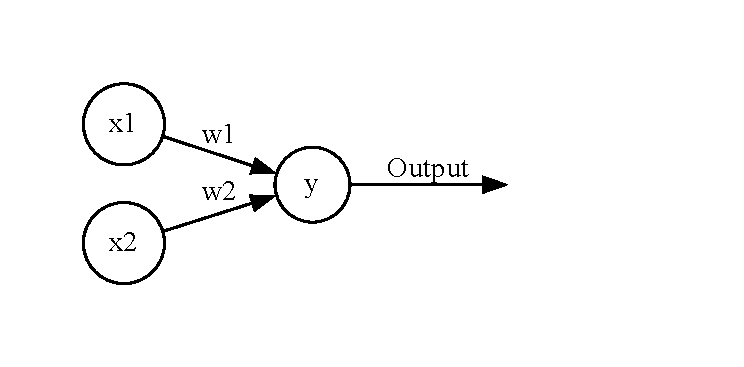
\includegraphics[width=0.5\textwidth]{graph/rosenblatt}
  \label{fig:perceptron}
\end{figure}

The second wave started in the early 1960ies with Rosenblatt's perceptron convergence theorem \cite{rosenblatt1962principles}. A visualization of the perceptron can be seen in \figureref{fig:perceptron} and the output of the perceptron is calculated as follows:
\[
    p(x)= 
\begin{cases}
    1, & \text{if } \sum_i w_ix_i + b > 0\\
    0, & \text{otherwise}
\end{cases}
\]
Setting $w1$ and $w2$ to 1 yields a perceptron that implements the logical or operation. As McCulloch and Pitts' work showed, the perceptron is able to model all simple logical operations such as: and, or, not. However the second wave slowed as Minsky and Papert showed that the perceptron is unable to model the XOR operation \cite{minsky1969perceptron} even though the \ac{MLP} that Rosenblatt already proposed at the time could model XOR through the combination of multiple perceptrons \cite{schmidhuber2022annotated}.

The third and ongoing wave started in the early 1980ies with Hopfield's energy approach \cite{hopfield1982neural} as well as the introduction and refinement of back-propagation for \acp{MLP} \cite{werbos1974beyond,rumelhart1986parallel}.

\subsection{CNN}

\begin{figure}
  \caption{Visualization of a \ac{MLP}}
  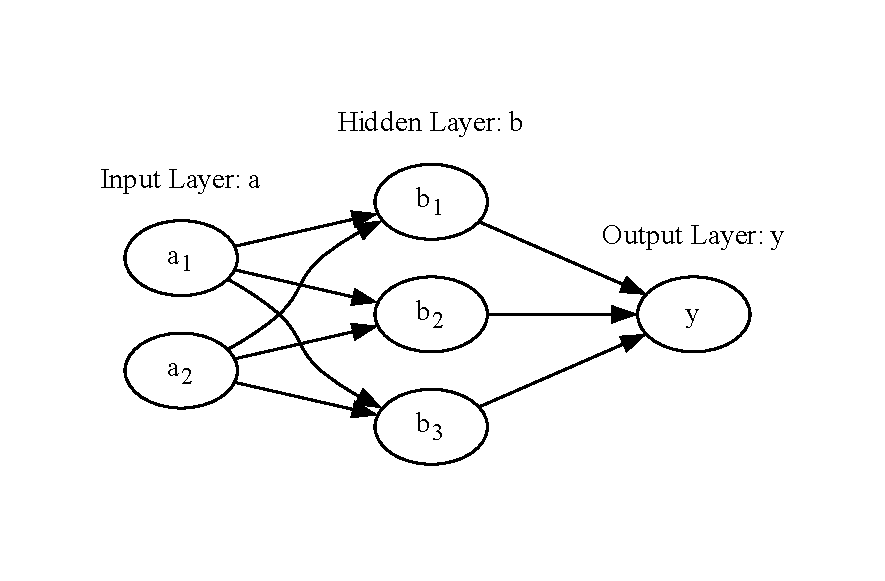
\includegraphics[width=0.5\textwidth]{graph/mlp}
  \label{fig:mlp} 
\end{figure}

Each node in b in the \ac{MLP} as seen in \figureref{fig:mlp} is calculated like the node y in \figureref{fig:perceptron}. That also means that every node combination between the layers has a weight. Such a combination of layers is called a fully connected layer. When there is a lot of correlation between all the nodes, then such a fully connected layer is useful as it is also fully utilized. However particularly when the nodes of the input layer represent the pixels of an image and the task is some form of recognition of objects in the image, most connections are not well utilized, since pixels that are further away from each other tend to have no meaningful connection \cite{aghdam2017guide}.

Convolutional layers work like a kernel based image filter but make the kernel trainable instead of static. This has the advantage that each convolutional neuron only processes data from its receptive field instead of the whole image. The receptive field of a neuron refers to the area of pixels in the source image that the data the neuron gets is dependent on. Using just one convolutional layer means that the neurons in the resulting tensor are just dependent on an area in the source image as big as the kernel of that convolution. Therefore \acp{CNN} tend to have many layers to be able to recognize larger shapes in the image. The resulting data of a convolutional layer is also called a feature map. 

\section{Shapely}

Shapely is a popular Python package for computational geometry. It provides a wide range of geometric objects and operations for working with planar geometric shapes, such as points, lines and polygons. Shapely is widely used in various domains, including geographic information systems (GIS), spatial data analysis, and computer graphics.

\section{Open CV}

\ac{OpenCV} is an open-source computer vision and machine learning software library designed for various computer vision tasks such as image processing, object detection, image recognition, and more. It was originally developed by Intel and later maintained by Willow Garage and Itseez. \ac{OpenCV} is written in C++ and has interfaces for C++, Python, and other programming languages, making it widely accessible and used in both academia and industry.

\subsection{ArUco Detection}

The \ac{ArUco} library implemented into \ac{OpenCV} is based on a paper from S. Garrido-Jurado et al. \cite{garrido2014automatic}. The \ac{ArUco} detection starts by using local adaptive thresholding on the image. Afterwards the Suzuki
and Abe algorithm \cite{SUZUKI198532} is applied to the thresholded image to extract the contours. The contours are then transformed into polygons \cite{douglas1973algorithms} and all polygons with more or less than 4 vertices are discarded. Then homographies for all remaining polygons are calculated such that the perspective on the potential marker is removed. The flattened image is then binarized using Otsu's method \cite{4310076}, which results in the lowest possible intra-class variance of black and white parts of the potential marker. Finally the marker is divided into a grid and further processed as a binary number based on the brightness of the grid cells.

This algorithm is however based on the assumption that the marker contour is always visible. If it isn't detections can become skewed or nothing is detected as seen in \figureref{fig:aruco-det}.

\begin{figure}
  \centering
  \subcaptionbox{An easily detectable \ac{ArUco} marker image}
     {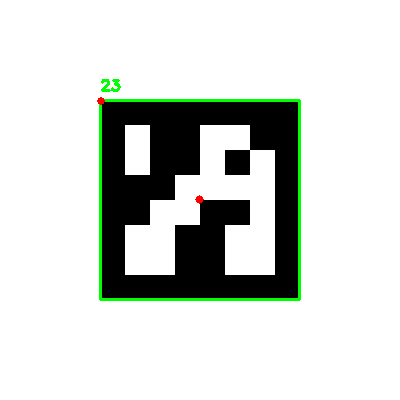
\includegraphics[width=0.3\textwidth]{image/rec}}
  \subcaptionbox{An \ac{ArUco} marker image with obscured contour corner}
     {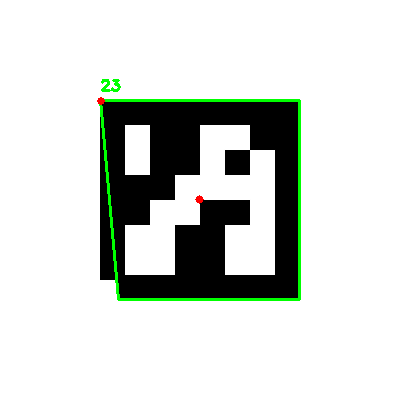
\includegraphics[width=0.3\textwidth]{image/skewed-rec}}
  \subcaptionbox{An \ac{ArUco} marker image with broken contour}
     {
\includegraphics[width=0.3\textwidth]{image/no-rec}}
  \caption{Open CV ArUco Detection on example \ac{ArUco} images which have been partly obscured by a white rectangle}
  \label{fig:aruco-det}
\end{figure}

\section{Albumentations}

Albumentations is a popular Python library for image augmentation, primarily designed for use in computer vision and deep learning tasks \cite{info11020125}. Image augmentation is a technique used to artificially expand a dataset by applying various transformations to the existing images. This helps improve the performance and generalization of machine learning models, especially in scenarios where the training data is limited.

\section{Pytorch}

PyTorch is an open-source machine learning library for Python that has gained significant popularity in the deep learning and artificial intelligence research communities. Originally developed by Facebook's AI Research lab (FAIR) and now maintained by the Linux Foundation, PyTorch offers a flexible and dynamic computational graph, making it particularly well-suited for developing and training neural networks.

\section{HyperOpt}

Hyperopt is a Python package designed for hyperparameter optimization, a fundamental aspect of machine learning model development \cite{bergstra2013making}. It systematically explores the hyperparameter space using a variety of optimization algorithms, most notably \ac{TPE}, aiming to discover the parameter combination that optimizes a predefined objective function. 

Hyperopt sees the objective function as a black box and makes few assumptions, which comes with flexibility but slower optimization than with loss functions in neural network training. Since the entire machine learning process is not a derivable function, this is the best choice for optimizing hyperparameters.

A combination of grid search and manual search are widely used to optimize hyperparameters. However it was shown that such processes tend to not be as efficient as sampling randomly from the hyperparameter space \cite{bergstra2012random}. \ac{TPE} is based on this realization as it behaves like random sampling in the first runs, but afterwards it uses the sampling history to find promising new parameter combinations \cite{bergstra2011algorithms}. 
% \ac{TPE} roughly works in these steps:

% \begin{enumerate}
%   \item Initialize the search space with Gaussian distributions or categorical distributions for continuous parameters and discrete parameters respectively.
%   \item Sample the objective function
%   \item The outputs of the objective function are thresholded into good and bad configurations
%   \item A exploitation \ac{PDF} is constructed for good configurations and a exploration \ac{PDF} is constructed for bad configurations
%   \item 
% \end{enumerate}

\section{mAP Scores}

\ac{mAP} scores are a class of commonly used metrics in the field of object detection to evaluate the performance of an object detection model \cite{padilla2020survey}. They aim to provide a measure of how well the model can identify and locate objects within an image. However there is a lack of consensus about the \ac{mAP} calculation. I will therefore focus on three popular \ac{mAP} scores. 

\subsection{IoU}

\begin{figure}
  \caption{Visualization of \ac{IoU} calculation}
  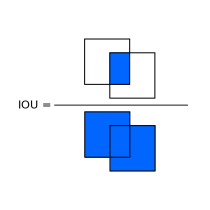
\includegraphics[width=0.5\textwidth]{image/iou}
  \label{fig:iou}
\end{figure}

The metric commonly chosen to measure the prediction quality between a prediction and ground truth label is the \ac{IoU} \cite{padilla2020survey}. The \ac{IoU} is a measurement based on the  Jaccard Index, a coefficient representing the similarity of two sets of data \cite{jaccard1901etude}. In the object detection context the \ac{IoU} measures the area of overlap divided by the area of union between two bounding boxes as shown in \figureref{fig:iou}.

\subsection{Precision and Recall}

In the context of object detection there exist three prediction cases, with the \ac{TN} case being omitted, since it applies to all possible bounding boxes that were not predicted, which depends more on the image resolution than the predictions, assuming the bounding box coordinates are integer values.

\begin{itemize}
  \item[$\bullet$] \ac{TP}: The highest confidence prediction of a ground truth label with an \ac{IoU} higher than the threshold
  \item[$\bullet$] \ac{FP}: An incorrect or imprecise prediction
  \item[$\bullet$] \ac{FN}: An undetected ground truth bounding box
\end{itemize}

Since \ac{TN} is not available in this context, metrics that use the \ac{TN} are also not available \cite{padilla2020survey}. Instead precision $P$ and recall $R$ are used as metrics.

$$P = \frac{TP}{TP + FP} = \frac{TP}{\text{all predictions}}$$

$$R = \frac{TP}{TP + FN} = \frac{TP}{\text{all ground truths}}$$

Precision measures the percentage of correct predictions among all predictions and recall measures the percentage of correct predictions among all ground truth boxes. 

The difference becomes most apparent when thinking about the extreme cases. If a model would output every possible bounding box on an image the recall would be 100\%, since for each ground truth bounding box there is an exact same prediction bounding box. If a model would instead output a perfect prediction for one ground truth bounding box and nothing for any other ground truth bounding boxes, the precision would be 100\%, since each made prediction is correct. Since both cases are undesirable but still result in an high score in one of the metrics a combination of both is needed.

\subsection{Table}

\begin{figure}
  \caption{Visualization of example prediction and ground truth bounding boxes}
  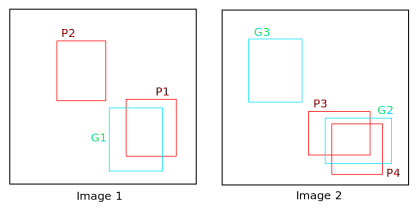
\includegraphics[width=0.8\textwidth]{image/preds}
  \label{fig:preds}
\end{figure}

The first part of the \ac{mAP} calculation are the same across all scores considered. That unified part of the computation is described here using the example\footnote{\url{https://kharshit.github.io/blog/2019/09/20/evaluation-metrics-for-object-detection-and-segmentation}, accessed on 08.10.2023} shown in \figureref{fig:preds}. 

Firstly a table of all predictions over all images in a given dataseries is created as seen in Table \ref{tab:mAP}. The table is sorted by prediction confidence. If there are multiple predictions for a single ground truth label, the prediction with the highest confidence is considered TP, if its \ac{IoU} is over the threshold, and all others FP, as seen with prediction P3. 

\begin{center}
  \begin{tabular}{ c c c c c c c c }
   Ground truth & Prediction & Confidence & TP & Acc. TP & Acc. FP & Precision & Recall \\ 
   \hline
   G2 & P4 & 98\% & Yes & 1 & 0 & 1 & 0.33 \\
   G2 & P3 & 89\% & No & 1 & 1 & 0.5 & 0.33 \\
   G1 & P1 & 78\% & Yes & 2 & 1 & 0.67 & 0.67 \\
   - & P2 & 60\% & No & 2 & 2 & 0.5 & 0.67 \\
   \hline
  \end{tabular}
  \label{tab:mAP}
\end{center}

As the table is stepped through from highest confidence predictions to lowest, the accumulated TP and FP are incremented based on whether the prediction was correct or incorrect and saved into each table row \cite{padilla2020survey}. By computing $\text{acc \ac{TP}} / (\text{acc \ac{TP}} + \text{acc \ac{FP}})$ a preliminary precision is computed for each row. Similarly a preliminary recall value is calculated for each table row by dividing the accumulated \ac{TP} by the total number of ground truth labels of all images. Its important to note that recall values due to their computation formula here are monotonically increasing as the table rows are visited. When plotting the precision and recall values of the table rows as y and x components of points, the \ac{PR curve} is obtained as seen in \figureref{fig:pr-curve}.

\begin{figure}
  \caption{Example of a \ac{PR curve} plot taken from training with real data}
  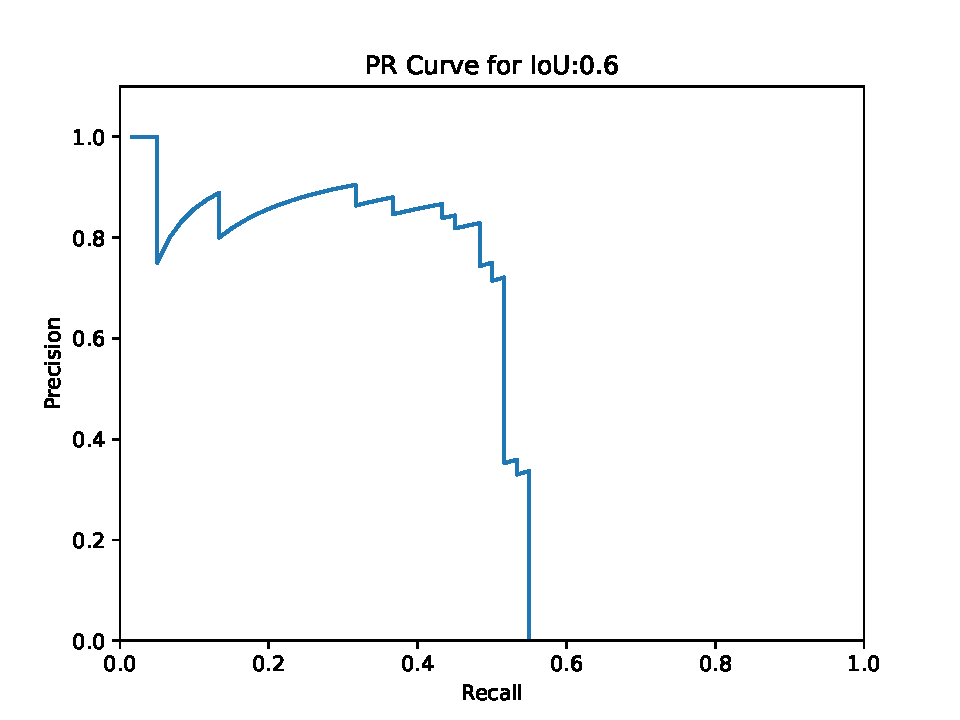
\includegraphics[width=0.8\textwidth]{image/eval_PR_Curve_0.60}
  \label{fig:pr-curve}
\end{figure}

The \ac{mAP} scores are now based on the \ac{AUC} of the \ac{PR curve}, which represents the desired combination of the precision and recall scores.

\subsection{Pascal VOC 2007}

For the VOC 2007 score the table as described earlier is computed for an \ac{IoU} threshold of 0.5 \cite{everingham2010pascal}. This threshold is deliberately set low to account for inaccuracies on the ground truth data, that can arise from hard to label objects. The VOC 2007 score summarizes the shape of the \ac{PR curve} by taking 11 equally spaced recall values . For each chosen recall value the maximum precision value on the curve at or to the right of that recall value is computed. Finally the AP score is defined as the mean of those maximum precision values as given by:

$$AP_{11} = \frac{1}{11} \sum_{r\in(0,0.1,...,1)}p_{interp}(r)$$

where

$$p_{interp}(r) = max_{\bar{r} : \bar{r} \geq r}p(r)$$

%$$p(r) = \text{the precision value on the \ac{PR curve} given a recall value}$$

Since I focus on the one class case for object detection eg. only on ArUco markers, that AP score is also the \ac{mAP} score here, otherwise the \ac{mAP} score would be the mean of the AP scores of all classes.

\subsection{Pascal VOC 2010}

The VOC 2010 score computes the \ac{PR curve} for an \ac{IoU} threshold of 0.5. It considers the \ac{PR curve} \ac{AUC} not just at 11 points but on all points of the table, giving this approach the name all-point interpolation \cite{padilla2020survey}. It is computed using the following formula:

$$AP_{all} = \sum_{n}(r_{n+1} - r_n)p_{interp}(r_{n+1})$$

where

$$p_{interp}(r_{n + 1}) = max_{\bar{r} : \bar{r} \geq r_{n+1}}p(\bar{r})$$

Since the VOC 2010 score takes all given recall values into account it is generally more accurate than the VOC 2007 score.

\subsection{COCO}

The object detection part of the COCO detection challenge defines multiple AP score types, such as AP across scales where the ground truth masks are split by their pixel area \cite{padilla2020survey}. However for this work I focused on the most used AP score definition of COCO, which is the AP@50:5:95 score. It refers to the computation of multiple \acp{PR curve} using different \ac{IoU} thresholds. In this case 10 \ac{IoU} thresholds from 0.50 to 0.95 with a step width of 0.05. COCO also uses recall points, similar to the VOC 2007 score. However with 101 values instead of 11 between 0 and 1 with a step width of 0.01. %given by the following number series: ${0, 0.01, ..., 1}$. 
The COCO mAP score then refers to the average of the computed mAP scores for each \ac{IoU} threshold. 

The COCO scores usefulness lies in its measurement of how tight a prediction bounding box is around a ground truth bounding box using higher \ac{IoU} thresholds. Both VOC scores described see a prediction as correct as soon as its \ac{IoU} is above 0.5 and make no difference between predictions with an \ac{IoU} of 0.55 or 0.9. The COCO score therefore gives the opportunity to measure further improvements to trained models, if the VOC scores are already high, assuming the ground truth labels of the dataset are accurate enough.

\chapter{Related Work}
\label{chap:relatedw}

\section{ArUco Marker Detection}

\section{Training Image Augmentations}

\section{Classic Detection Approaches?}

\chapter{Networks}
\label{chap:netw}

\section{Yolov5}

\section{Yolov8}

\section{YolovNAS}

\section{MobileNetV2}

\section{ViTs}

\chapter{Implementation}
\label{chap:implement}

\section{Used Hardware}

\section{Automated Annotations}

\section{Software Architecture}

\section{Augmentations}

\section{Synthetic Data}

\section{Plotting}

\section{Automated Evaluation of Multiple Ensemble Trainings}

\section{Hyperparameter Optimization}

\section{Point Detection}

\chapter{Evaluation}
\label{chap:eval}

\section{Test Data}

\section{Human Testing}

\section{Augmenting from Zero}

\section{Augmenting from Optimum}

\section{Discussion}

%\subsection{Confusion Matrix in Object Detection}

\chapter{Conclusion}
\label{chap:conclusion}

\section{Summary}

\section{Future Work}

\subsection{Deploying on Mobile}

\subsection{Tracking}

\chapter{Appendix}

\section{List of Abbreviations}

\begin{acronym}
% From bachelor thesis
\acro{GUI}{Graphical User Interface}
\acro{UI}{User Interface}
\acro{JSON}{JavaScript Object Notation}
\acro{SVG}{Scalable Vector Graphics}
\acro{LMB}{left mouse button}
\acro{AABB}{Axis Aligned Bounding Box}
\acroplural{AABB}{Axis Aligned Bounding Boxes}
\acro{HTML}{Hypertext Markup Language}
\acro{GIMP}{GNU Image Manipulation Program}

% From Fabio
\acro{POC}{Point-of-care}
\acro{POCT}{Point-of-care Testing Device}
\acro{IBE}{ion beam etching}
\acro{PCS}{Photonic Crystal Slab}

% From master thesis
\acro{ArUco}{Augmented Reality University of Cordoba}
\acro{GPU}{Graphics Processing Unit}
\acro{ANN}{artificial neural network}
\acro{NN}{neural network}
\acro{MLP}{multilayer feedforward network}
\acro{CNN}{convolutional neural network}
\acro{OpenCV}{Open Source Computer Vision Library}
\acro{TPE}{Tree-structured Parzen Estimators}
\acro{PDF}{probability density function}
\acro{mAP}{mean Average Precision}
\acro{IoU}{intersection over union}
\acro{PR curve}{precision recall curve}
\acro{TP}{true positive}
\acro{FP}{false positive}
\acro{FN}{false negative}
\acro{TN}{true negative}  
\acro{AUC}{area under the curve }

\end{acronym}

\section{User Evaluation Files}


\backmatter
\tocbibliography

\end{document}